\documentclass[paper=letter, fontsize=11pt]{scrartcl} % A4 paper and 11pt font size
\newcommand{\horrule}[1]{\rule{\linewidth}{#1}} % Create horizontal rule command with 1 argument of height
\setlength{\parskip}{1em}
\setlength{\parindent}{3em}
\usepackage{listings}

\usepackage{hyperref}
\usepackage{enumerate}
\usepackage{amsmath}
\usepackage{geometry}
 \geometry{
 bottom=1in,
 right=1in,
 left=1in,
 top=1in,
 }

 \usepackage[flushleft]{threeparttable}
\usepackage[capposition=top]{floatrow}

\usepackage{graphicx}
 \graphicspath{ {../figures/} }

\title{	
\normalfont \normalsize 
\horrule{0.5pt} \\[0.4cm] % Thin top horizontal rule
 \large{{\textbf{ECON 293 Homework 1: Commentary}}} \\ % The assignment title
\horrule{2pt} \\[0.5cm] % Thick bottom horizontal rule
}

\author{\small{Jack Blundell, Spring 2017}} % Your name

\date{} % Today's date or a custom date

\begin{document}

\maketitle % Print the title

In this commentary I discuss results and include some key figures. Many further figures and all code are provided in the attached .html file. I worked with Luis Armona on the code. This commentary is written individually.

\section{Randomized Control Trial}

We chose to use data from ``Does Price Matter in Charitable Giving?
Evidence from a Large-Scale Natural Field Experiment", by Dean Karlan and John List (AER 2007). In this experiment, two-thirds of recipients of a charity solicitation letter receive some kind of match-donation treatment, whereas the remaining control group receives the letter alone, with no matching promise. There are a total of $50,082$ participants. 

First we estimate the average treatment effect, pooling all treatments, on our outcome variable for which we use total donation given. We estimate this via simple regression, finding a treatment effect of $0.1536$, with a 95\% confidence interval of $-0.0082, 0.3154 $, consistent with the results in the paper.

\section{Emulating a Quasi-experiment via Selection}

Our selection rule uses the fact that in the paper, estimated treatment effects are highest among states which voted for Bush in the 2004 presidential election, and that this effect is biggest for the most marginal states. The probability of selection conditional on treatment allocation and covariates $Pr(S|W,X)$ is chosen to be:
\[
  Pr(S|W,X)= \begin{cases}
  	  (.01 + -0.01 ihs(X_{3})^5 + ihs(X_{3})^3)/300 & \text{if $W=1$} \\
	  (X_{2}+1) (\arccos(X_{1}) \arctan(X_{1}) )/3 & \text{if $W=0$} \\ 
     0.5 & \text{if missing one of } X_{1},X_{2},X_{3}
      \end{cases} 
\]
Here, $W$ is treatment, $X_1$ is the percentage who voted for Bush in the 2004 presidential election, and $X_1,X_2$ are other covariates found to be correlated with treatment effects. $ihs$ is the inverse hyperbolic sine function (e.g. $ihs(X) = \log(X_{3} + \sqrt{X_{3} ^ 2 + 1}$). For those with missing values of these covariates, the probability of inclusion in the sample is one half. The above selection rule is a highly non-linear function involving several variables and hence unlikely to be recoverable by standard propensity score methods. 

Figure \ref{select_c} shows the shape of this function across proportion of Bush voters for a number of other covariate values for the control group. Figure \ref{select_t} shows the same for the treatment group, this time with the x axis as the value of the highest previous donation, one of our other covariates on which selection is based. These selection rules are designed to disproportionately sample those in the treatment group with high treatment effects, in a complex non-linear way.

\begin{figure}[!ht]
\center
\caption{  \label{select_c}}
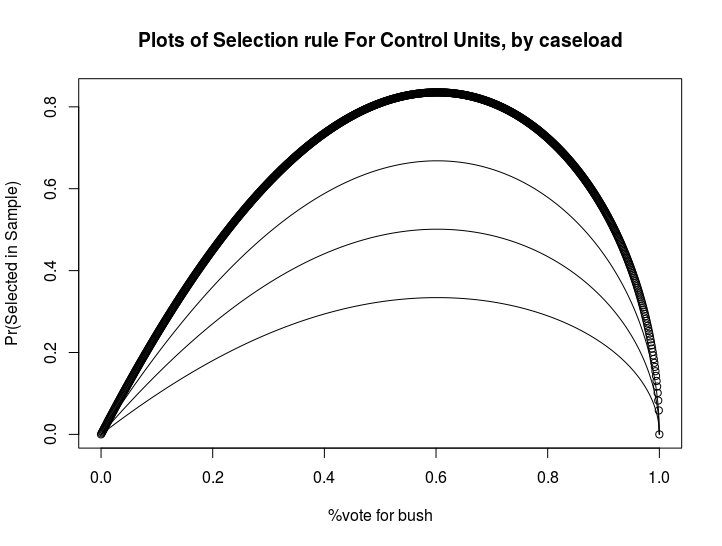
\includegraphics[scale=0.8]{select_c.png}
\floatfoot{Notes: x-axis is number of votes won by Bush in previous election. This graph shows the shape of our selection rule for the control group across a number of different covariate values.}
\end{figure}

\begin{figure}[!ht]
\center
\caption{  \label{select_t}}
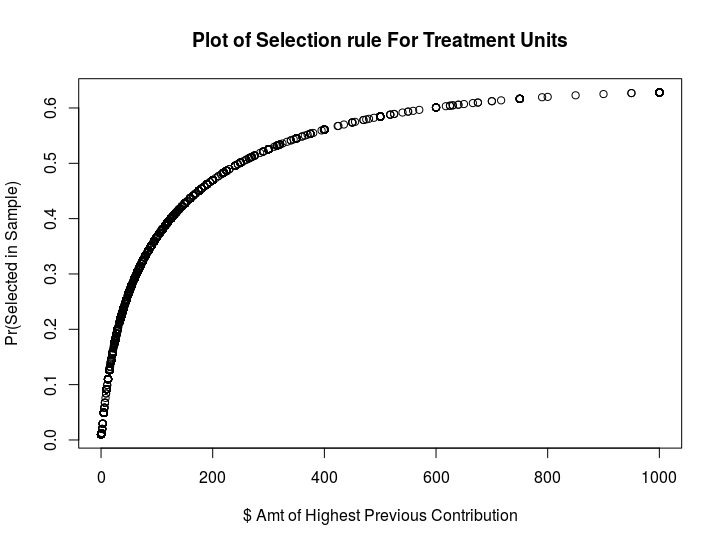
\includegraphics[scale=0.8]{select_t.png}
\floatfoot{Notes: x-axis is highest previous donation to charity. This graph shows the selection rule for the treatment group.}
\end{figure}

We calculate $Pr(S|W,X)$ for each observation, and use a uniform random number generator to drop observations based on this. This selection means that we no-longer have a randomized experiment. After this censoring process, we are left with $15,167$ observations. Table \ref{treat} shows the full set of treatment effects estimated in this homework. The first row shows the simple OLS on the full sample discussed in the above section. This could be considered the `true' treatment effect, i.e. the estimated treatment effect without selection. This is what we will seek to recover with all methods in this homework. 

In row (2), we run simple OLS on the censored sample, estimating a treatment effect of $0.4027$. When we restrict the sample according to our selection rule, the estimated treatment effect increases dramatically. Our selection rule has resulted in selection into treatment based on high treatment effects and hence simple or `naive' OLS is biased.

\begin{table}[htbp]  \small
 \centering
  \begin{threeparttable}  
\caption{Estimated treatment effects \label{treat}}\begin{tabular}{l*{1}{c}}
\hline
Estimator           &     Estimated ATE     
\rule{0pt}{4ex}  \\
\hline\hline 
(1) Full-sample simple OLS (\textit{`true' ATE}) &  0.1536 \rule{0pt}{4ex} \\

(2) Restricted-sample simple OLS &  0.4027  \\ \hline
(3) PS Weighting          &            0.2685 \rule{0pt}{4ex} \\
(4) OLS with Controls       &            0.1961 \\ 
(5) Traditional DR OLS with IPS Weights & 0.1752\\ \hline 
(6) Regularized PS Weighted &             0.2764  \rule{0pt}{4ex} \\
(7) DR OLS with Regularized IPS Weights & 0.2300 \\ 
(8) Direct LASSO on Outcome &   0.2283 \\   \hline
(9) Double Selection       &    0.2026 \rule{0pt}{4ex} \\
(10) LASSO Residual-on-Residual & 0.2269 \\
(11) Residual balancing & 0.2462 \\
\end{tabular}
\begin{tablenotes}
\item Notes: This table shows the various treatment effects estimated throughout this homework
    \end{tablenotes}
  \end{threeparttable}
\end{table}

Overlap is demonstrated in Figure \ref{overlap}, which shows the CDFs of true propensity scores for the treatment and control groups in the restricted sample.

\begin{figure}[!ht]
\center
\caption{Overlap  \label{overlap}}
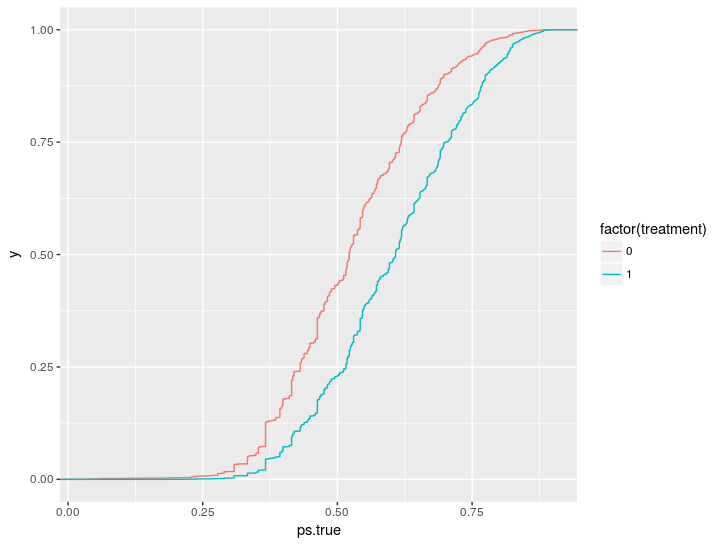
\includegraphics[scale=0.8]{overlap.png}
\floatfoot{Notes: This graph shows the CDF of the true propensity scores among treatment and control groups.}
\end{figure}

These true propensity scores are calculated by Bayes theorem, combining our selection rule with the (unconditional) probability of treatment in the original sample. Recalling that $S$ is the event that an observation is selected, the propensity score is:
\begin{align*}
P(W=1|S,X) &= \frac{P(S|W=1,X)P(W=1) }{P(S|W=1,X)P(W=1) + P(S|W=0,X)P(W=0)}
\end{align*}
For those with missing covariates, the propensity score equals 2/3, which is the same as the unconditional treatment probability.

Figure \ref{bias} is the histogram of the bias function as given in Athey, Imbens, Pham and Wager (2017). Since our selection rule involves continuous covariates, in calculating the bias function we calculate outcome means within neighborhoods of observations. We determine these neighborhoods by the minimum Mahalanobis distance needed to include at least one treatment and one control, standardizing covariates to have mean 0 and variance 1. The expected bias is $0.0441$. As expected, since we have disproportionately included the treated with high treatment effects, the bias is generally positive. If we were to treat this as a random experiment, our treatment effect estimate would be biased upwards. This is consistent with what we see in the first two rows of Table \ref{treat}.

\begin{figure}[!ht]
\center
\caption{Bias Function  \label{bias}}
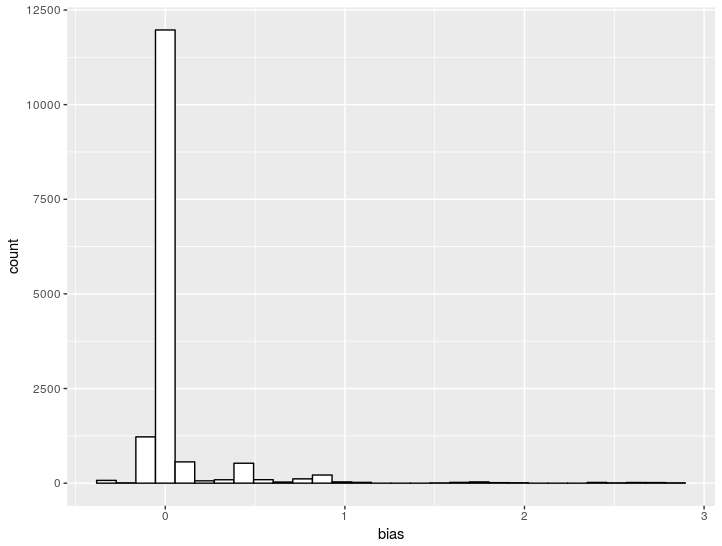
\includegraphics[scale=0.8]{bias.png}
\floatfoot{Notes: This graph shows the distribution of the bias, as given in Athey, Imbens, Pham and Wager (2017).}
\end{figure}

\section{Alternative methods to recover the ATE}

As we saw in the previous section, treating our modified dataset as if treatment has been allocated randomly leads to an upwardly-biased estimate. Here we attempt a number of different methods to attempt to account for the non-random selection into treatment. Throughout, our feature space ($X$) includes all covariates and two-way interactions, bar covariates indicating missing values.

\subsection{Standard methods}

Rows (3) - (5) for Table \ref{treat} represent standard econometric approaches to recovering the ATE when using observational data in a non-randomized experiment. Row (3) shows the estimate when we use propensity score weighting. To calculate this, we estimate the propensity score via a linear regression of treatment on the full feature space, which allows us to predict the probability of treatment $\hat{e}(X)$. The propensity-score weighted ATE is then given by:

\[\widehat{ATE}_{PS} = \frac{1}{N}\sum_i \frac{ Y_i(W_i-\hat{e}(X))}{\hat{e}(X_i)(1-\hat{e}(X_i)) }\]

We see the estimate is $0.2685$. The propensity score weighting does better than the simple OLS of row (2), but is still far from the estimate we are trying to recover in row (1).

In row (4), we use multivariate regression on the treatment and the full feature space. This does substantially better than propensity score weighting, giving an estimate of $0.1961$. In row (5), we use `double-robust' OLS in which we run OLS with inverse propensity score weights $w_i$, where:
\[w_i = \frac{1}{W_i\hat{e}(X_i) + (1-W_i)(1-\hat{e}(X_i))}\]

This again delivers an improvement, producing an estimate of $0.1752$. In fact, this is the method that comes closest to recovering the \textit{`true'} ATE of row (1). All in all then, we see that the conventional methods do a reasonable job at accounting for non-random assignment, making big gains over our initial naive simple OLS approach.

\subsection{ML methods}

In rows (6) - (8) we apply a number of modern Machine-Learning style methods to attempt to uncover the ATE. First, in row (6) we use a propensity score method just as above, but instead of OLS to estimate the propensity score, we use LASSO. Here we choose 10-fold cross validation, as is standard, to select the regularization parameter based on lowest mean squared error. Once we have our new $\hat{e}(X)^{LASSO}$, the procedure is identical to the standard PS weighting described above. Since estimating the propensity score is essentially a prediction problem, we might hope that LASSO would improve on OLS by preventing overfitting. We see that using LASSO to estimate the propensity score does worse that the standard propensity score weighting, with an estimate of $0.2764$. To understand why this is the case, in Figure \ref{pscore} we show a density comparison of the true, OLS and LASSO propensity scores. We see that LASSO is far less smooth, in a sense attempting to fit the non-linearities in the true propensity score, but doing so somewhat unsuccessfully. The OLS-estimated propensity score misses many of the non-linearities, but captures the general shape far better. From this figure then, it is not all that surprising that the LASSO-estimated propensity scores to not deliver good estimates.

\begin{figure}[!ht]
\center
\caption{Comparison of propensity scores  \label{pscore}}
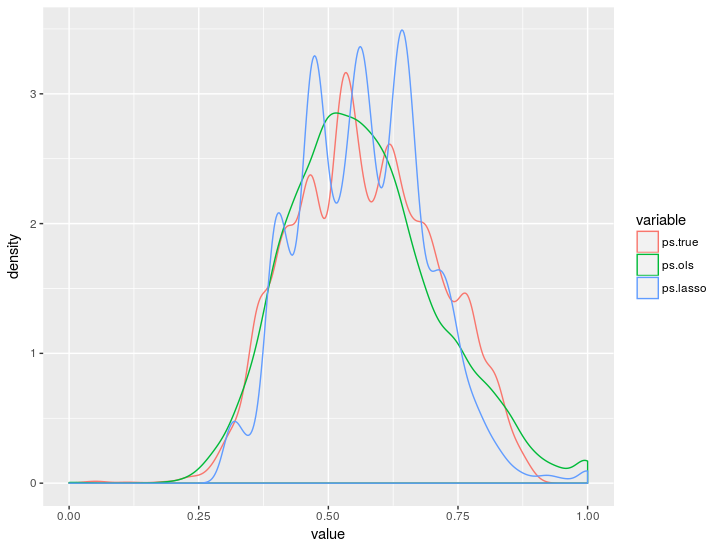
\includegraphics[scale=0.8]{pscore_ests.png}
\floatfoot{Notes: This graph shows the densities of the true, OLS and LASSO propensity scores.}
\end{figure}

Next we use double robust methods but using our lasso-estimated propensity scores to calculate the IPS weights, giving an estimate of $0.2300$. Although this improves on the lasso propensity score weighted estimate, again this is inferior to the standard version due to the poor estimation of propensity scores.

Finally for this set of methods, in column (8) we use a LASSO regularized regression directly on our treatment and full feature space. We set the penalty factor on treatment to zero so as not to penalize this estimated coefficient. We find a treatment effect of $0.2283$.  This is the best of this set of methods, but still does poorly relative to the conventional ones of the previous section.

In Figure \ref{lasso_coef} we show our estimated treatment coefficient as a function of the penalty factor $\lambda$. We see that as the penalty becomes greater, the estimated treatment effect increases, converging to the simple OLS estimate of $0.4027$ as all other coefficients are pushed towards zero. Intuitively, the more we penalize coefficients, the less we can account for selection into treatment. We see when $\lambda=0$, the treatment coefficient coincides with that of (unregularized) OLS with controls. Cross validation selects a $\lambda$ approximately equal to 0.1. We also plot the paths of many other coefficients, which I omit here and leave in the attached markdown file.

\begin{figure}[!ht]
\center
\caption{Estimated LASSO Treatment Effect and Regularization  \label{lasso_coef}}
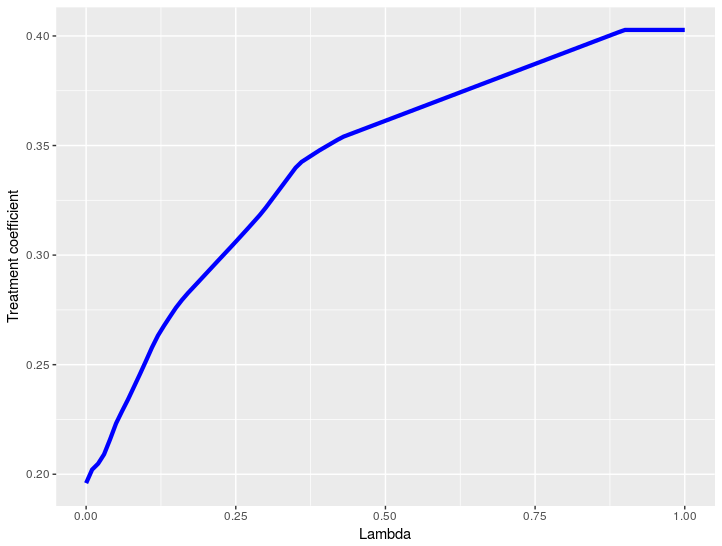
\includegraphics[scale=0.8]{treat_coef_lasso.png}
\floatfoot{Notes: This graph shows how the estimated treatment effect varies with penalty factor $\lambda$.}
\end{figure}

\section{Further Machine Learning methods}

Here we present the results from three more ML-style approaches. The first is the double-selection method given in Belloni, Chernozhukov and Hansen (2014). In this method, we use lasso both to select variables from the propensity equation and from the outcome equation. We then running OLS including as controls the variables which are selected by both. As shown in row (9) in Table \ref{treat}, this delivers and estimate of $0.2026$. We find this to be the best among the ML methods, although still not as good as OLS with the full set of controls.

Next we use double machine learning, or LASSO residual-on-residual. In this method we run LASSO regressions of $Y$ on $W$ and $W$ on $X$, before running a simple OLS regression of the residuals of the former on those of the latter. This gives an estimate of $0.2269$, which is reasonably poor.

Finally, we use balanceHD for approximate residual balancing, delivering an estimate of $0.2462$. This is something of a poor performance relative to other methods. We believe this may be connected to issues in applying the algorithm in the package to large problems. 

\subsection{Discussion}

Overall, comparing all results in Table \ref{treat}, the winner of our comparison exercise here is traditional double-robust OLS with inverse propensity score weights. In general, traditional methods out-performed the more complex ML methods. We hypothesize that this will often likely be the case in observational studies where the feature space is small relative to the number of observations. After our feature engineering of creating interactions, we are left with approximately 300 covariates, which is relatively small for a sample of over 10,000 observations. In a setting with far more covariates, the benefits of ML would perhaps result in superior performance relative to conventional methods.

We have learned from this project that one must think carefully about which method is appropriate for each individual setting, and that there is no one-size-fits-all method. In this case, and particularly given the additional complexity and computational load of the ML methods, the traditional methods from econometrics have won the day.

\end{document}
